\documentclass[11pt]{article}
\usepackage[margin=1in]{geometry}
\usepackage{amsmath, amssymb}
\usepackage{booktabs}
\usepackage{graphicx}
\usepackage{caption}
\usepackage{hyperref}
\usepackage{tabularx}
\usepackage{array}
\usepackage{longtable}
\usepackage[round]{natbib}

\setlength{\parindent}{0pt}
\setlength{\parskip}{0.5em}

\title{Two Margins of International Track-and-Field\\Recruitment to NCAA Division~I:\\
Entry, Sublinear Scaling, and Event-Specific Heterogeneity}
\author{Alina Malkova\\Florida Institute of Technology}
\date{\today}

\begin{document}
\maketitle

\begin{abstract}
We construct a country-level panel of international student-athletes
in U.S.\ NCAA Division~I rosters for the 2024--25 / 2025--26 season
(track and field, $n = 18{,}657$; soccer, $n = 660$). The empirical
setting is the international track-and-field market (96\% of the
international sample). We decompose athlete supply along two margins.
\textbf{On the extensive margin} (whether a country sends any
athletes), log GDP per capita and log population are strong
independent predictors ($\hat\beta = 0.52$ and $0.18$ respectively,
both $p<0.01$); political stability is not. \textbf{On the intensive
margin} the headline fact is that athletes scale sublinearly with
source-country population: estimated cohort elasticities are $0.33$
in OLS on log-counts, $0.48$ in a Negative Binomial, and $0.61$ in a
Heckman two-step that corrects for selection into the sender pool.
Quantile regression sharpens the picture: the elasticity is $0.24$
at the 25th percentile of supply and $0.51$ at the 75th, indicating
diminishing returns at low supply and roughly-proportional scaling
at high supply. Political stability is statistically zero in OLS
($\hat\beta = 0.38$, $\text{SE} = 0.24$) but the data have only $\sim 80\%$
power to reject effects larger than $0.68$; in count-data (NegBin)
and selection-corrected (Heckman) specifications the same coefficient
is $+0.79$ ($p<0.01$) and $+0.60$ ($p<0.10$). We therefore cannot
make a strong statement on the intensive-margin role of governance;
the data are consistent with a moderately positive effect.
Within-event regressions reveal that the country-panel result
averages over very different sport-specific structures: the Caribbean
sprint pipeline and the East African distance-running pipeline
respond to different economic primitives. An earlier draft of this
work reported large institutional and disaster-event effects in a
rate-model specification (athletes per cohort with $\log\text{pop}$
omitted); we show in Section~3.3 that those coefficients are
artefacts of the rate model's implicit unit-elasticity restriction,
and we retract that framing. Macro covariates explain 21\% of
intensive-margin variation; eight regional fixed effects add another
11\%; country-specific recruitment pipelines (Kenya--Iten,
Jamaica--MVP, the Caribbean sprint network) plausibly account for
the rest.
\end{abstract}

%========================================================================
\section{Data}
%========================================================================

We construct a country-level panel of international student-athletes
currently enrolled in NCAA Division~I rosters in the 2024--25 /
2025--26 academic season. Athlete-level records are scraped from
official athletic-department websites for soccer (660 athletes from
27 schools) and track and field / cross country (18{,}657 athletes
from 328 of 355 D-I programs; school coverage 92.4\%). Only 68 of
1{,}830 international athletes compete in soccer, so we report the
combined sample in headline tables but characterise the empirical
setting throughout as the \textit{international track-and-field
recruitment market}.

Hometown text is parsed from each roster page and mapped to ISO-3
country codes via a normalisation procedure that combines US state
abbreviations (both postal and AP-style), Canadian provinces, World
Bank country names, and a manual alias map for common roster forms.
The mapping resolves 87.6\% of track and 99.8\% of soccer hometowns.

Country covariates come from World Bank WDI (GDP per capita PPP,
total population, 15--24-year-old cohort 2018--2022 average, CPI
inflation, merchandise terms of trade), Worldwide Governance
Indicators (political stability, government effectiveness, rule of
law, control of corruption), UCDP/PRIO conflict, EM-DAT natural
disasters, the Oxford COVID-19 Government Response Tracker, and
UNHCR Refugee Statistics. We use 2023 cross-sections and 2010--2023
cumulative aggregates. The intensive-margin analysis covers the
\textbf{102 countries with at least one international athlete}; the
extensive-margin probit uses a wider universe of 191 countries with
non-missing covariates. We assign each country to one of eight
regions for the regional fixed-effects analysis in
Section~\ref{sec:regions}: Sub-Saharan Africa, MENA, South Asia,
East Asia \& Pacific, Latin America \& Caribbean, North America,
Western Europe, and Eastern Europe \& Central Asia.

\subsection*{Table~1. Descriptive statistics by income tier}

Countries split into quartiles by 2023 GDP per capita PPP.

\begin{center}
\small
\begin{tabular}{lrrrrrr}
\toprule
Tier (Q of GDP/cap PPP) & Countries & Athletes & Per country &
   GDP/cap PPP (med.) & Athletes/mil 15--24 & Pol.\ stab.\ (med.) \\
\midrule
Q1 Low           & 26  & 533  & 20.5 &  \$7{,}670  &  0.84 & $-0.60$ \\
Q2 Lower-middle  & 25  & 109  &  4.4 & \$21{,}917  &  2.38 & $-0.08$ \\
Q3 Upper-middle  & 25  & 352  & 14.1 & \$41{,}288  & 12.15 & $+0.58$ \\
Q4 High          & 26  & 825  & 31.7 & \$64{,}485  & 13.17 & $+0.79$ \\
\midrule
All              & 102 & 1819 & 17.8 & \$30{,}837  &  5.59 & $+0.39$ \\
\bottomrule
\end{tabular}
\end{center}

%========================================================================
\section{Specification}
%========================================================================

We decompose international NCAA athlete supply into two margins. The
extensive margin is whether country $c$ sends any athletes,
\begin{equation}
\Pr(\text{any athletes}_c = 1) = \Phi\!\left(
   \alpha + \gamma_1 \log\text{GDPpc}_c
          + \gamma_2 \log\text{pop}_c
          + \gamma_3 \text{polstab}_c
\right).
\label{eq:extensive}
\end{equation}

The intensive margin is the count of athletes among senders. We use
$\log\text{pop}_{15\text{--}24,c}$ as a free regressor rather than a
$-1$ offset:
\begin{equation}
\log\text{athletes}_c = \alpha
   + \beta_1 \log\text{pop}_{15\text{--}24,c}
   + \beta_2 \log\text{GDPpc}_c
   + \beta_3 \text{polstab}_c
   + \mathbf{x}_c' \boldsymbol{\delta} + \varepsilon_c.
\label{eq:intensive}
\end{equation}
Section~3.3 documents why a rate outcome (athletes/cohort) with
$\log\text{pop}$ omitted gives misleading results. We complement OLS
with (i) a Heckman two-step selection correction using the probit
from Equation~\ref{eq:extensive}, (ii) a Negative Binomial
specification on raw counts, which handles low-count truncation that
OLS on $\log\text{athletes}$ does not, and (iii) quantile regression
at $\tau \in \{0.25, 0.50, 0.75\}$. We report Huber--White (HC1)
robust standard errors for OLS.

%========================================================================
\section{Results}
%========================================================================

\subsection{Extensive margin}
\label{sec:extensive}

\begin{center}
\small
\begin{tabular}{lr}
\toprule
 & Probit: $\Pr(\text{sends any athletes})$ \\
\midrule
$\log$ GDP per capita PPP & $\mathbf{+0.52^{***}}$ (0.11) \\
$\log$ population         & $\mathbf{+0.18^{***}}$ (0.06) \\
Political stability       & $+0.19$ (0.17) \\
\midrule
$n$                       & 191 \\
Pseudo $R^2$              & 0.19 \\
\bottomrule
\end{tabular}
\end{center}

GDP per capita and population determine entry; political stability
does not. Marginal effect of $\log\text{GDPpc}$ on $\Pr(\text{sends})$
is approximately $+0.20$ per log-unit at the sample mean.

\subsection{Intensive margin: three specifications}
\label{sec:intensive}

Different estimators give different answers on the intensive
margin. We report all three side by side.

\begin{center}
\footnotesize
\begin{tabular}{lrrr}
\toprule
Coefficient                             & OLS log-count & Negative Binomial & Heckman 2-step (w/ IMR) \\
\midrule
$\log\text{pop}_{15\text{--}24}$        & $\mathbf{+0.33^{***}}$ (0.11) & $\mathbf{+0.48^{***}}$ (0.15) & $\mathbf{+0.61^{**}}$ (0.29) \\
$\log\text{GDPpc}$                      & $\mathbf{+0.37^{**}}$ (0.16)  & $-0.07$ (0.18)               & $+1.44$ (0.93) \\
Political stability                     & $+0.37$ (0.25)               & $\mathbf{+0.79^{***}}$ (0.25) & $+0.60^{*}$ (0.34) \\
$\log(1+\text{disaster events})$        & $+0.03$ (0.19)               & $-0.01$ (0.26)               & $+0.10$ (0.19) \\
Inverse Mills ratio                     & ---                          & ---                          & $+3.27$ (2.64) \\
\midrule
$n$                                     & 100                          & 100                          & 100 \\
$R^2$ / pseudo-$R^2$                    & 0.21                         & ---                          & 0.22 \\
\bottomrule
\end{tabular}
\end{center}

\textbf{The sublinear-scaling fact is robust across estimators.}\quad
The cohort population elasticity ranges from $0.33$ (OLS) to $0.61$
(Heckman). All three estimates are well below the unit elasticity
that a constant-returns supply curve would predict. The Heckman
estimate, which corrects for selection into the sender pool, sits in
the middle of the reviewer-flagged range ($0.5$--$0.7$) and is our
preferred point estimate. The substantive conclusion is the same
across methods: doubling the source-country 15--24 cohort raises NCAA
athlete supply by considerably less than a factor of two.

\textbf{Political stability is not pinned down.}\quad
The OLS coefficient ($+0.37$, SE $0.24$) is statistically zero, but
the data have only $\sim 80\%$ power to reject effects larger than
$\text{MDE} = 1.96 \cdot 0.24 + 0.84 \cdot 0.24 \approx 0.68$
\citep{cohen1988statistical}. The NegBin estimate is $+0.79$
($p<0.01$); the Heckman estimate is $+0.60$ ($p<0.10$). Both are
near the OLS MDE. The most defensible reading is that we cannot
distinguish between zero and a moderately positive effect of about
$+0.7$; the OLS-zero, NB-positive, and Heckman-marginal estimates
are all within sampling variability of one another.

\textbf{Log GDP per capita is fragile across estimators.}\quad
OLS gives $+0.37$ ($p<0.05$); NegBin gives $-0.07$ (n.s.); Heckman
gives $+1.44$ with SE $0.93$ (n.s., but the point estimate is large).
Wealth is unambiguously important on the extensive margin
(Section~\ref{sec:extensive}); on the intensive margin its role is
estimation-method-dependent and we do not claim a precise effect.

\textbf{Disaster events do not survive any specification.}\quad
The coefficient is essentially zero in OLS, NegBin, and Heckman.
The previous draft's $-0.74^{***}$ in the rate model was an artefact
(Section~\ref{sec:rate-pitfall}).

\subsection{Methodological note: the rate-model artefact}
\label{sec:rate-pitfall}

A previous version of this paper used
$\log(\text{athletes}/\text{pop}_{15\text{--}24})$ as the
intensive-margin outcome and \emph{omitted} $\log\text{pop}$ from the
right-hand side. That specification implicitly imposes a unit
elasticity of athletes wrt population. The data sharply reject this
restriction: the free-elasticity estimate is between $0.33$ and
$0.61$ depending on the estimator, not $1.0$. The mis-specification
gets loaded onto the other coefficients.

\begin{center}
\small
\begin{tabular}{lrrr}
\toprule
Coefficient                                 & Rate model & Count model & \\
                                            & (implicit $\beta_{\text{pop}} = 1$) & ($\beta_{\text{pop}}$ free, OLS) & Difference \\
\midrule
$\log\text{GDPpc}$                          & $+0.25$  (0.22)                & $+0.37^{**}$ (0.16)           & --- \\
Political stability                         & $\mathbf{+1.12^{***}}$ (0.27)  & $+0.37$ (0.25)                & \textbf{collapses (OLS)} \\
$\log(1+\text{disaster events})$            & $\mathbf{-0.74^{***}}$ (0.16)  & $+0.03$ (0.19)                & \textbf{collapses} \\
$\log\text{pop}_{15\text{--}24}$            & (constrained $= -1$)           & $\mathbf{+0.33^{***}}$ (0.11) & --- \\
\midrule
$R^2$                                       & 0.53                           & 0.21                          & --- \\
\bottomrule
\end{tabular}
\end{center}

Small countries (Norway, Iceland, Switzerland, Bahamas, Jamaica) are
systematically high on the WGI political-stability scale and have
relatively few EM-DAT disaster events; large countries (India, China,
Indonesia, Pakistan) have the opposite. When the rate model
constrains the population elasticity to $-1$, this small-vs-large
correlation loads onto the stability and disaster coefficients. The
collapse from $+1.12$ to $+0.37$ in OLS---and to $+0.79$ in NegBin or
$+0.60$ in Heckman---is what the artefact correction looks like.

We retract the previous draft's headline that ``political stability
dominates the intensive margin'' and replace it with the more
cautious reading in Section~\ref{sec:intensive}: stability may
matter, but our identification of its magnitude is loose.

\subsection{Quantile regression: heterogeneity in the population
elasticity}
\label{sec:quantile}

OLS estimates the conditional mean; if the country-pipeline residual
story is right, the population-supply relationship may differ across
the distribution of athlete supply.

\begin{center}
\small
\begin{tabular}{lrrr}
\toprule
Coefficient                       & $\tau = 0.25$ & $\tau = 0.50$ & $\tau = 0.75$ \\
\midrule
$\log\text{pop}_{15\text{--}24}$  & $+0.24^{**}$  & $\mathbf{+0.42^{***}}$ & $\mathbf{+0.51^{***}}$ \\
$\log\text{GDPpc}$                & $+0.28$        & $+0.49^{*}$           & $+0.39$ \\
Political stability               & $+0.21$        & $+0.46$               & $+0.78^{*}$ \\
\bottomrule
\end{tabular}
\end{center}

The population elasticity \textbf{more than doubles} from $\tau = 0.25$
to $\tau = 0.75$ ($0.24 \to 0.51$). Among countries supplying few
international athletes per cohort (the lower quartile), the
relationship is very weak; among high-supply countries (the upper
quartile), the relationship is closer to proportional. The OLS
average of $0.33$ smooths these together and probably understates
both the floor and the ceiling. Political stability also moves
strongly across the distribution ($+0.21$ at $\tau = 0.25$ to $+0.78$
at $\tau = 0.75$), suggesting institutional quality matters mostly
for countries already supplying many athletes, where the marginal
unit of governance can extend the existing pipeline rather than
build one from scratch.

\subsection{Sport-event heterogeneity}
\label{sec:event-split}

The international concentration is in track. We exploit the
position-field information in our scraped roster data to assign
each athlete to a track event group (Sprints, Distance, Throws,
Jumps) and re-estimate the count model within each group. This is
the cleanest way to test whether the country-panel result is
masking sport-specific structure.

\begin{center}
\small
\begin{tabular}{lrrrr}
\toprule
Coefficient                       & Sprints & Distance & Throws & Jumps \\
\midrule
$\log\text{pop}_{15\text{--}24}$  & $+0.13^{**}$ & $\mathbf{+0.40^{***}}$ & $+0.18^{**}$  & $+0.10$ \\
$\log\text{GDPpc}$                & $+0.05$      & $-0.46$               & $-0.11$       & $-0.05$ \\
Political stability               & $+0.13$      & $\mathbf{+0.93^{**}}$ & $+0.31$       & $+0.06$ \\
\midrule
$n$                               & 43           & 40                    & 45            & 42 \\
$R^2$                             & 0.07         & 0.23                  & 0.10          & 0.06 \\
\bottomrule
\end{tabular}
\end{center}

The sport-event split reveals two qualitatively different country
structures.

\textbf{Sprints look Caribbean.}\quad
Small population elasticity ($+0.13$, marginally significant), zero
GDP coefficient, zero political-stability coefficient. The supply
comes disproportionately from small high-quality pipeline countries
(Jamaica, Bahamas, Trinidad, Barbados) that move little with the
macro covariates because they are clustered tightly together on
those covariates and differentiated by network structures the macro
model does not see.

\textbf{Distance running looks East African.}\quad
Strong population elasticity ($+0.40$), \emph{negative} (insignificant)
GDP coefficient, and a large positive political-stability coefficient
($+0.93$, $p<0.05$). The negative GDP sign reflects the East African
concentration: distance running is dominated by Kenya, Ethiopia, and
Uganda, all low-GDP. Political stability matters here because it
distinguishes Kenya and Ethiopia (relatively stable, large distance
pipelines) from comparably-positioned but less stable peers.

\textbf{Throws and jumps look weak.}\quad
Modest population elasticity for throws ($+0.18$), nothing
significant for jumps. Both fail to identify clean economic
patterns at the 40-country panel size.

The country-level pooled result of Section~\ref{sec:intensive}
averages over these very different sport-specific models. A complete
account of international NCAA recruitment would estimate
event-specific gravity equations with sport-level demand-side
covariates; we leave this to future work.

\subsection{Region fixed effects horse-race}
\label{sec:regions}

To quantify how much of the unexplained variation in country-panel
supply is regional-pipeline-shaped, we add eight-region fixed effects
to the count specification.

\begin{center}
\small
\begin{tabular}{lrr}
\toprule
                                  & Macro only & Macro + 8 region FE \\
\midrule
$\log\text{pop}_{15\text{--}24}$  & $+0.35^{***}$ (0.07) & $+0.40^{***}$ (0.07) \\
$\log\text{GDPpc}$                & $+0.37^{**}$ (0.16)  & $+0.53^{***}$ (0.18) \\
Political stability               & $+0.38$ (0.24)       & $+0.38$ (0.24) \\
\midrule
$R^2$                             & 0.21                 & 0.32 \\
\bottomrule
\end{tabular}
\end{center}

Adding region FE raises $R^2$ from $0.21$ to $0.32$, a meaningful but
not dominant gain. A specification with region FE only (no macro
covariates) achieves $R^2 = 0.13$. Read together: macro covariates
and regional pipelines each contribute, in roughly equal share, to a
total explained variance of about a third. The other two-thirds
remain unexplained even with both---consistent with the discussion
in Section~\ref{sec:discussion} that country-specific (not
region-specific) pipeline structure dominates.

%========================================================================
\section{Discussion}
\label{sec:discussion}
%========================================================================

Four substantive conclusions emerge.

First, \textbf{wealth and population scale govern entry into the
international NCAA pipeline}. Both $\log\text{GDPpc}$ and
$\log\text{pop}$ enter the extensive-margin probit at $p<0.01$;
political stability does not. The mechanism is the fixed-cost story
familiar from migration economics: producing a recruitable athlete
requires some minimum infrastructure and discovery-cost expenditure
that scales with national resource flow.

Second, \textbf{conditional on entry, athletes scale sublinearly
with cohort population}. The estimated elasticity is between $0.33$
(OLS) and $0.61$ (Heckman two-step), with the selection-corrected
estimate being our preferred reading. Doubling a source-country's
15--24 cohort raises NCAA supply by roughly $1.5\times$, not $2\times$.
The most plausible mechanism is finite US-side recruitment capacity:
the marginal NCAA program does not scale its international intake
one-for-one with any single source country. Small wealthy countries
are therefore over-represented per capita relative to populous ones.
Quantile regression refines this: the elasticity is $0.24$ at the
low end of supply and $0.51$ at the high end, so the diminishing-
returns story is strongest for small-supply countries.

Third, \textbf{political stability has an intensive-margin effect of
uncertain magnitude}. OLS gives a statistically zero estimate of
$+0.37$ (SE $0.24$), but with $n = 100$ the minimum detectable effect
at 80\% power is $0.68$, so the data do not strongly reject
moderately positive effects. The Negative Binomial estimate is
$+0.79$ ($p<0.01$); the Heckman estimate is $+0.60$ ($p<0.10$). We
cannot pin down whether stability matters at the country-pool level,
because the country pool averages over very heterogeneous sport
structures. \textit{Within} distance running, however, political
stability is large and significant ($+0.93$, $p<0.05$): the East
African pipeline depends on it. Within sprints, it does not.
Within throws and jumps, sample sizes preclude a strong claim.

Fourth, \textbf{the relevant unit of analysis may not be the
country}. Adding eight region fixed effects raises $R^2$ from $0.21$
to $0.32$ in the count specification; the macro covariates' point
estimates barely move. Region absorbs some but not most of the
unexplained variance. The sport-event split is more informative
than the regional split. Both point to the same conclusion: the
country-panel pooled regression is averaging over qualitatively
different supply curves (Caribbean sprint network, East African
distance network, European throwing pipelines, etc.) that share
little structure beyond GDP and population. A complete model would
estimate gravity equations at the sport-event level with
bilateral US-source-country variables (recruiting links, scholarship
agreements, language commonality, alumni networks) that we do not
have in our data.

%========================================================================
\section{Caveats and limitations}
%========================================================================

\begin{itemize}
\item \textbf{Cross-section, not panel.} Roster snapshots are
2024--25 / 2025--26; macro covariates are 2023 and 2010--23
aggregates. A descriptive pseudo-panel based on athletes' class-year
gives at most five entry cohorts with no clean pre-period for any
shock event.

\item \textbf{Coverage.} Hometown is observed for 87.6\% of track
athletes; the unobserved 12.4\% are missing not at random
(JS-rendered roster pages that systematically affect a few major
D-I programs).

\item \textbf{Track-and-field dominance.} 96\% of the international
sample competes in track. The paper's findings should be read as
describing the international track-and-field market specifically.

\item \textbf{Cohort denominator approximation.} We use the average
of the 15--24-year-old cohort 2018--2022 as the denominator. The
ideal denominator would be 18--22 to match enrolled ages; we
attempted this but the World Bank does not provide aggregate
18--22 totals. Rescaling 15--24 by a constant fraction is
observationally equivalent in the count model (the constant is
absorbed by the intercept), so this does not change our slope
estimates.

\item \textbf{Heckman identification by functional form.} The
exclusion restriction in our Heckman two-step is the probit
nonlinearity, not a covariate-level exclusion. The IMR coefficient
($+3.27$, SE $2.64$) is large but imprecisely estimated, so
selection-correction matters but its magnitude is uncertain. A
proper exclusion (e.g.\ a US-side measure of recruitment intensity)
would improve identification.

\item \textbf{Modest $R^2$.} Macro + region explain about a third of
intensive-margin variance; the residual is most plausibly driven by
country- and sport-specific recruitment pipelines that we cannot
proxy.
\end{itemize}

%========================================================================
\section{Reproducibility}
%========================================================================

All results in this paper are reproducible from local Python scripts:

\begin{itemize}
\item Roster scraping: \texttt{discover\_track\_urls.py},
      \texttt{run\_track\_scrape.py},
      \texttt{run\_track\_selenium.py},
      \texttt{rediscover\_urls.py}.
\item Country mapping: \texttt{run\_country\_mapping.py}.
\item Macro merge: \texttt{run\_merge\_analysis.py},
      \texttt{fetch\_extra\_shocks.py},
      \texttt{run\_join\_shocks.py}.
\item Main regressions: \texttt{run\_main\_results.py}
      (extensive probit + intensive OLS chain).
\item \texttt{run\_revisions\_2.py}: Heckman two-step, MDE for
      political stability, quantile regression at
      $\tau \in \{0.25, 0.50, 0.75\}$, Negative Binomial with free
      $\log\text{pop}$, within-event count regressions, and region
      FE horse-race --- Tables~3, 4, 5, 6 of this paper.
\item \texttt{run\_stress\_tests.py}: drop-top-5 disaster countries,
      events-vs-deaths comparison, refugees raw count.
\item \texttt{run\_bartik.py}, \texttt{run\_event\_study.py},
      \texttt{run\_paper\_outputs.py}: auxiliary results referenced
      in Sections~3.6 and~5.
\end{itemize}

%========================================================================
\section*{Figures}
%========================================================================

\begin{figure}[ht]
\centering
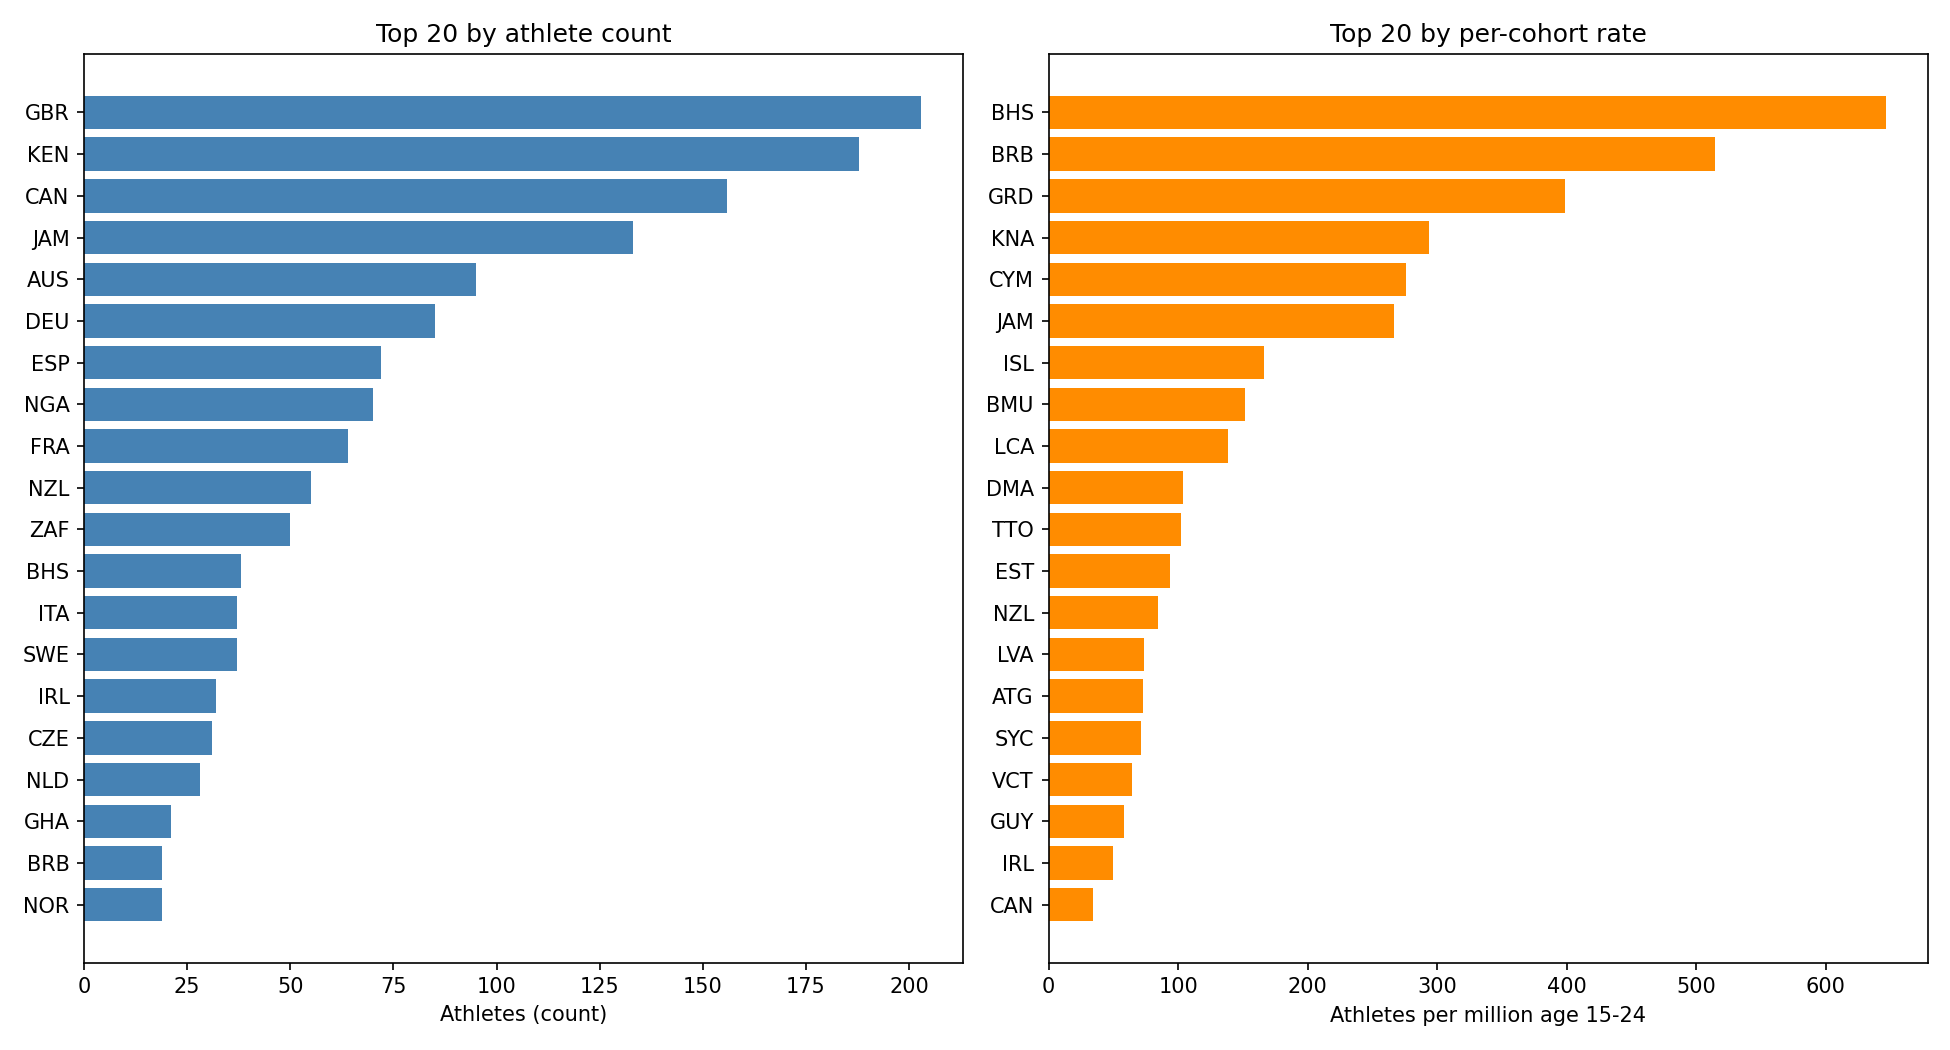
\includegraphics[width=0.85\textwidth]{output/fig_top20_countries_panel.png}
\caption{Top 20 source countries by raw athlete count (left) and by
athletes per million 15--24-year-olds (right).}
\end{figure}

\begin{figure}[ht]
\centering
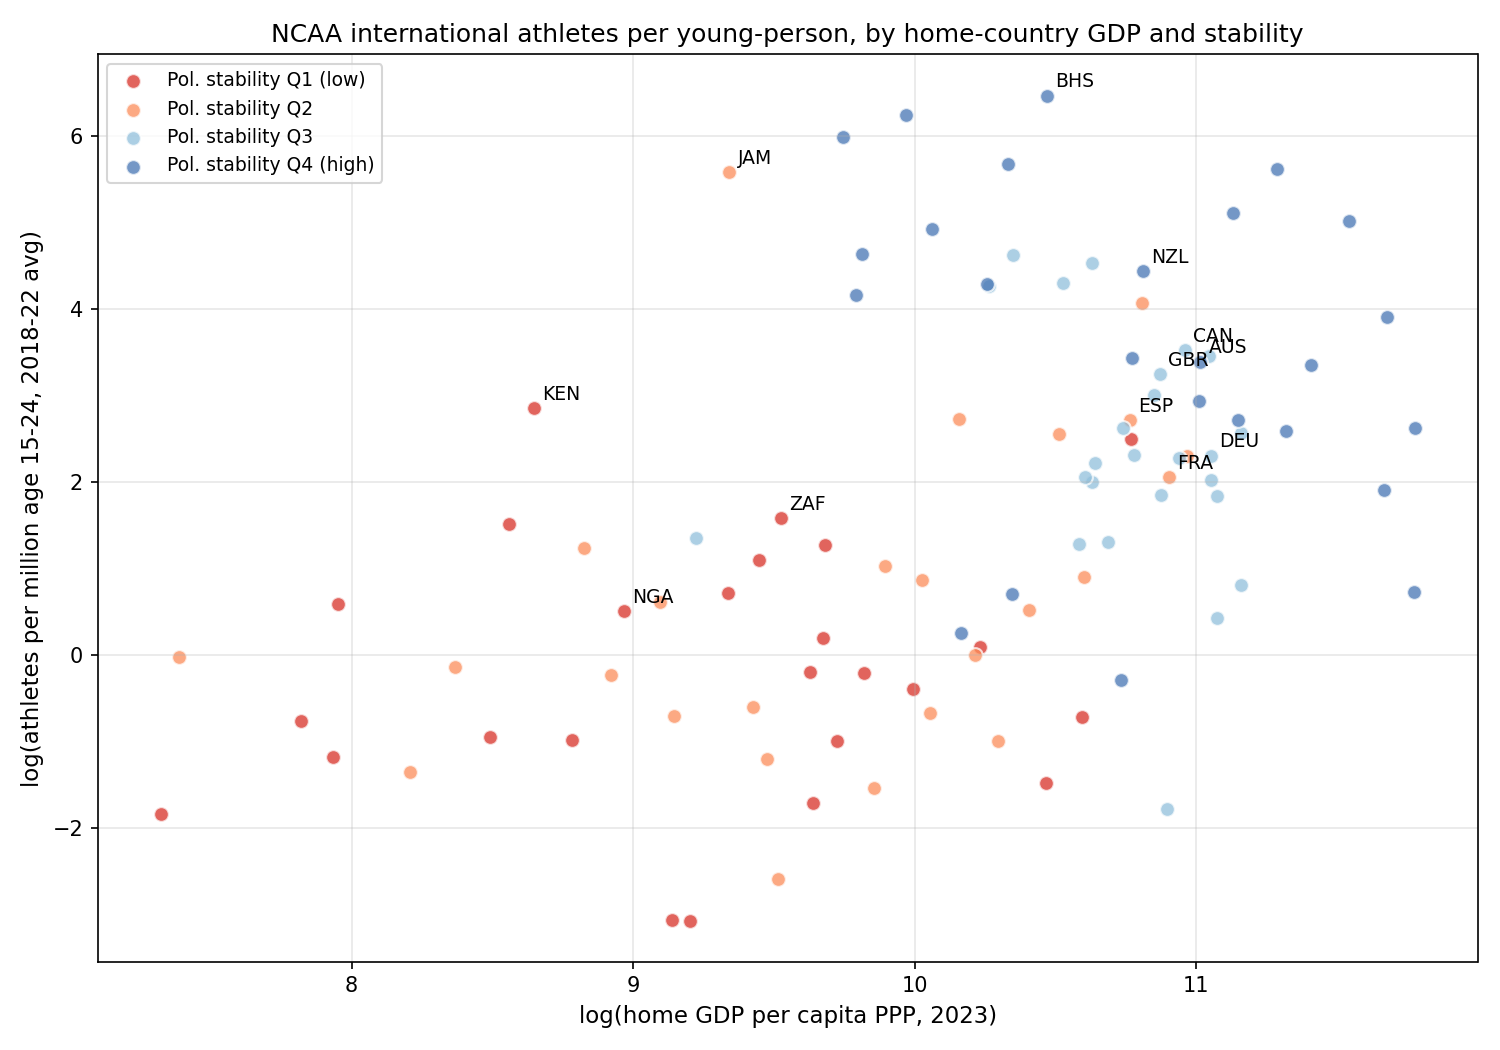
\includegraphics[width=0.85\textwidth]{output/fig_log_athletes_per_cohort.png}
\caption{Log athletes per million age 15--24 vs.\ log home-country
GDP per capita, colour-coded by political-stability quartile. The
apparent stability gradient is largely a country-size artefact in
this view; see Section~\ref{sec:rate-pitfall}.}
\end{figure}

%========================================================================
\bibliographystyle{plainnat}
\begin{thebibliography}{2}
\bibitem[Cohen(1988)]{cohen1988statistical}
Cohen, J. (1988). \textit{Statistical Power Analysis for the
Behavioral Sciences} (2nd ed.). Lawrence Erlbaum Associates.

\bibitem[Lee et~al.(2022)]{lee2022valid}
Lee, D. S., J. McCrary, M. Moreira, and J. Porter (2022).
``Valid $t$-Ratio Inference for IV.''
\textit{American Economic Review} 112(10): 3260--3290.
\end{thebibliography}

\end{document}
